\documentclass[11pt,a4paper]{article}

\usepackage[a4paper,
            top=25mm, bottom=25mm,
            left=25mm, right=25mm,
            headheight=15pt]{geometry}

\usepackage[utf8]{inputenc}
\usepackage{amsmath,amssymb}
\usepackage{graphicx}
\usepackage{booktabs}
\usepackage{hyperref}
\usepackage[dvipsnames]{xcolor}
\usepackage{tikz}
\usetikzlibrary{arrows.meta,decorations.pathreplacing,patterns,calc}
\usepackage[numbers,sort&compress]{natbib}
\usepackage{fancyhdr}
\usepackage{microtype}
\usepackage{siunitx}
\usepackage{listings}
\usepackage{caption}

\pagestyle{fancy}
\fancyhf{}
\lhead{\small SAMBP TR-12/2026 --- 87L Magnitude Override}
\rhead{\small PhD Thesis Supporting Report}
\cfoot{\thepage}

\hypersetup{colorlinks=true, linkcolor=blue!70!black, citecolor=OliveGreen,
            urlcolor=blue!70!black}

\newcommand{\sambp}{\textsc{sambp}}
\newcommand{\Idiff}{I_{\mathrm{diff}}}
\newcommand{\Ifund}{I_{\mathrm{fund}}}
\newcommand{\fint}{f_{\mathrm{int}}}
\newcommand{\alphaThresh}{\alpha_{\mathrm{thresh}}}
\newcommand{\alphafifty}{\alpha_{50}}
\newcommand{\kappan}{\kappa_n}
\newcommand{\eps}{\varepsilon}

\lstset{basicstyle=\ttfamily\small,
        keywordstyle=\color{blue!70!black},
        commentstyle=\color{gray},
        frame=single, breaklines=true}

%=======================================================================
\begin{document}
%=======================================================================

\begin{center}
  {\LARGE\bfseries SAMBP Technical Report TR-12/2026}\\[6pt]
  {\large 87L Line Differential: Magnitude Override for\\
          High-Impedance Fault Sensitivity Recovery}\\[4pt]
  \today
\end{center}

\vspace{4pt}
\noindent\rule{\linewidth}{0.6pt}

\begin{abstract}
SAMBP TR-11 identified a sensitivity penalty in the 87L line differential
relay under high-impedance fault (HIF) conditions: the Stage-2 model veto
suppressed correct conventional trips when the fault current fell below
$\alpha \approx 0.15$ (ag) or $0.07$ (3ph) of nominal, because low fault current
reduces the LM-estimated fundamental $\Ifund$ below the $\fint$ trip
threshold.  This report extends the magnitude-override mechanism introduced
for the bus differential gate in TR-10 to the 87L confidence gate.  A
threshold of $\Ifund \geq 0.30$~pu is used to bypass the Stage-2 veto when
the conventional relay has already picked up.  Post-fix validation with
$N=200$ trials per scenario shows the 87L $\alphafifty$ improving from
$0.15\to0.10$ (ag) and $0.07\to0.05$ (3ph).  All bus and transformer zones
retain TPR\,=\,1.000 across all $\alpha \in [0.05, 1.00]$, confirming no
regression.
\end{abstract}

\noindent\rule{\linewidth}{0.6pt}

\tableofcontents
\vspace{6pt}

%=======================================================================
\section{Background and Motivation}
\label{sec:background}
%=======================================================================

The SAMBP Stage-2 confidence gate was designed to suppress spurious
conventional differential trips that arise from degraded measurement
conditions (synchronisation error, CT saturation, channel skew).  The gate
evaluates two quantities derived from the Levenberg--Marquardt (LM) parameter
estimator:
\begin{itemize}
  \item $\kappan$ — normalised condition number of the Jacobian; low values
        indicate an identifiable LM solution.
  \item $\fint$ — internal-fault fraction; a scalar in $[0,1]$ synthesised
        from the ratio of estimated fundamental current $\Ifund$ to the
        zone-specific fault threshold.
\end{itemize}

The veto fires when
\begin{equation}
  \kappan < \kappa_{\mathrm{thresh}}
  \quad\text{AND}\quad
  \fint < f_{\mathrm{int,thresh}},
  \label{eq:veto_base}
\end{equation}
indicating that the estimator is confident but has identified a
non-internal current profile.

TR-10 showed that under CT saturation the veto inadvertently blocked
\emph{genuine} internal trips on the 87B bus zones, because saturation
compresses the measured differential waveform and thus lowers $\fint$.  The
fix was a \emph{magnitude override}: if the estimated $I_{\mathrm{diff,fund}}$
exceeded 0.60~pu the veto was bypassed, since external faults cannot produce
a large sustained fundamental differential~\cite{SAMBP_TR10}.

TR-11 identified the same mechanism at play in the 87L line zone under HIF
conditions~\cite{SAMBP_TR11}.  At reduced fault levels ($\alpha \leq 0.15$
for ag faults, $\alpha \leq 0.07$ for 3ph faults) the LM solution becomes
low-SNR: $\Ifund$ falls below the zone's fault threshold (0.20~pu) and $\fint$
drops below 0.50, triggering the veto even though the fault is internal.
The conventional relay, which has a lower effective pickup, correctly trips
at all tested $\alpha$ values — but the Stage-2 gate suppresses it.

The present report implements the TR-11 Recommendation~1: extend the
magnitude override to \texttt{line\_confidence\_gate.py}.

%=======================================================================
\section{Design of the 87L Magnitude Override}
\label{sec:design}
%=======================================================================

\subsection{Discriminant selection}

For the 87L zone the relevant magnitude estimate is $\Ifund$, the LM-estimated
fundamental component of the \emph{differential} current (stored in
\texttt{LineZoneState.I\_fund}).  The discriminant logic mirrors TR-10:
\begin{itemize}
  \item \textbf{Through-fault + channel skew}: $\Ifund$ is small (skew
        amplitude $\leq 0.15$~pu in the simulation model).  Veto is correct
        and should fire.
  \item \textbf{Sync error}: $\Ifund$ is moderately elevated (0.05--0.15~pu)
        but below fault level.  Veto is correct.
  \item \textbf{HIF internal fault}: $\Ifund$ rises with fault current.  At
        $\alpha = 0.10$ (ag), $\Ifund \approx I_{f,\mathrm{nom}} \times \alpha
        = 4.8 \times 0.10 = 0.48$~pu — well above the override threshold.
\end{itemize}

\subsection{Threshold selection}

The override threshold $\Ifund \geq \theta_{\mathrm{ov}}$ must satisfy two
constraints simultaneously:
\begin{enumerate}
  \item $\theta_{\mathrm{ov}} > I_{\mathrm{fund,max}}^{\mathrm{non\text{-}fault}}$:
        comfortably above the maximum $\Ifund$ seen in non-fault conditions
        (sync error, skew) to avoid false overrides.
  \item $\theta_{\mathrm{ov}} < I_{\mathrm{fund,min}}^{\mathrm{HIF}}$: below the
        minimum $\Ifund$ at the lowest target detection level.
\end{enumerate}

From the TR-11 data and simulation model:
\begin{align}
  I_{\mathrm{fund,max}}^{\mathrm{non\text{-}fault}} &\approx 0.15\;\text{pu} \\
  I_{\mathrm{fund,min}}^{\mathrm{HIF}} \;\text{at } \alpha=0.10,\,\text{ag}
    &\approx 0.48\;\text{pu}
\end{align}

A threshold of $\theta_{\mathrm{ov}} = 0.30$~pu provides a factor-of-two
margin on both sides and is identical to the threshold applied in the 87B
gate normalised to the line-zone current scale.

\subsection{Implementation}

The modified veto logic in \texttt{evaluate\_87L\_confidence\_gate()} is:

\begin{lstlisting}[language=Python]
# Magnitude override: if I_fund is large, the fault is internal
# -- do not let low f_int suppress the trip.
magnitude_override = (
    zone_state.I_fund >= gate_cfg.veto_override_I_thresh
    and conventional_trip
)

model_vetoes_conventional = (
    gate_cfg.model_veto_enable
    and kn < gate_cfg.kappa_thresh
    and f_int < gate_cfg.f_int_thresh
    and not magnitude_override       # <-- new guard
)
\end{lstlisting}

The new field \texttt{veto\_override\_I\_thresh} defaults to 0.30~pu and is
added to \texttt{LineConfidenceGateConfig}.  No other changes are made to the
gate logic, confirmation counter, or sync-error handling.

\subsection{Asymmetry relative to the 87B gate}

The 87B gate uses \texttt{I\_diff\_fund} with a threshold of 0.60~pu.  The
87L gate uses \texttt{I\_fund} (same physical quantity, different field name)
with a threshold of 0.30~pu.  The lower threshold reflects the 87L zone's
lower nominal fault current and smaller restraint currents; the bus zones see
larger fault contributions from multiple feeders so the absolute magnitude
threshold is proportionally higher.

%=======================================================================
\section{Validation Results}
\label{sec:results}
%=======================================================================

The HIF sweep from TR-11 was re-run using \texttt{run\_hif\_study.py}
with the updated \texttt{line\_confidence\_gate.py}.  All parameters
($N = 200$, seed 2026, jitter $\pm5\%$, $\alpha \in [0.05, 1.00]$) are
identical to TR-11 to enable a direct comparison.

\subsection{87L line zone}

\begin{figure}[h]
  \centering
  % fig_87l_override_comparison.tex  —  87L TPR before vs after magnitude override
% Left: ag fault   Right: 3ph fault
% Solid blue = conventional, dashed red = SAMBP pre-TR-12, dotted green = SAMBP post-TR-12
% Alpha levels: 1.00 0.70 0.50 0.30 0.20 0.15 0.10 0.07 0.05
% X mapping: alpha*8  (alpha=1 → x=8, alpha=0.05 → x=0.4)
%
% ag data:
%   alpha:      1.00 0.70 0.50 0.30 0.20 0.15 0.10 0.07 0.05
%   conv:       1    1    1    1    1    1    1    1    1
%   pre-TR12:   1    1    1    1    1    0    0    0    0   (blind alpha<=0.15)
%   post-TR12:  1    1    1    1    1    1    0.175 0   0   (alpha50=0.10)
%
% 3ph data:
%   alpha:      1.00 0.70 0.50 0.30 0.20 0.15 0.10 0.07 0.05
%   conv:       1    1    1    1    1    1    1    1    1
%   pre-TR12:   1    1    1    1    1    1    1    0    0   (blind alpha<=0.07)
%   post-TR12:  1    1    1    1    1    1    1    1    0   (alpha50=0.05)
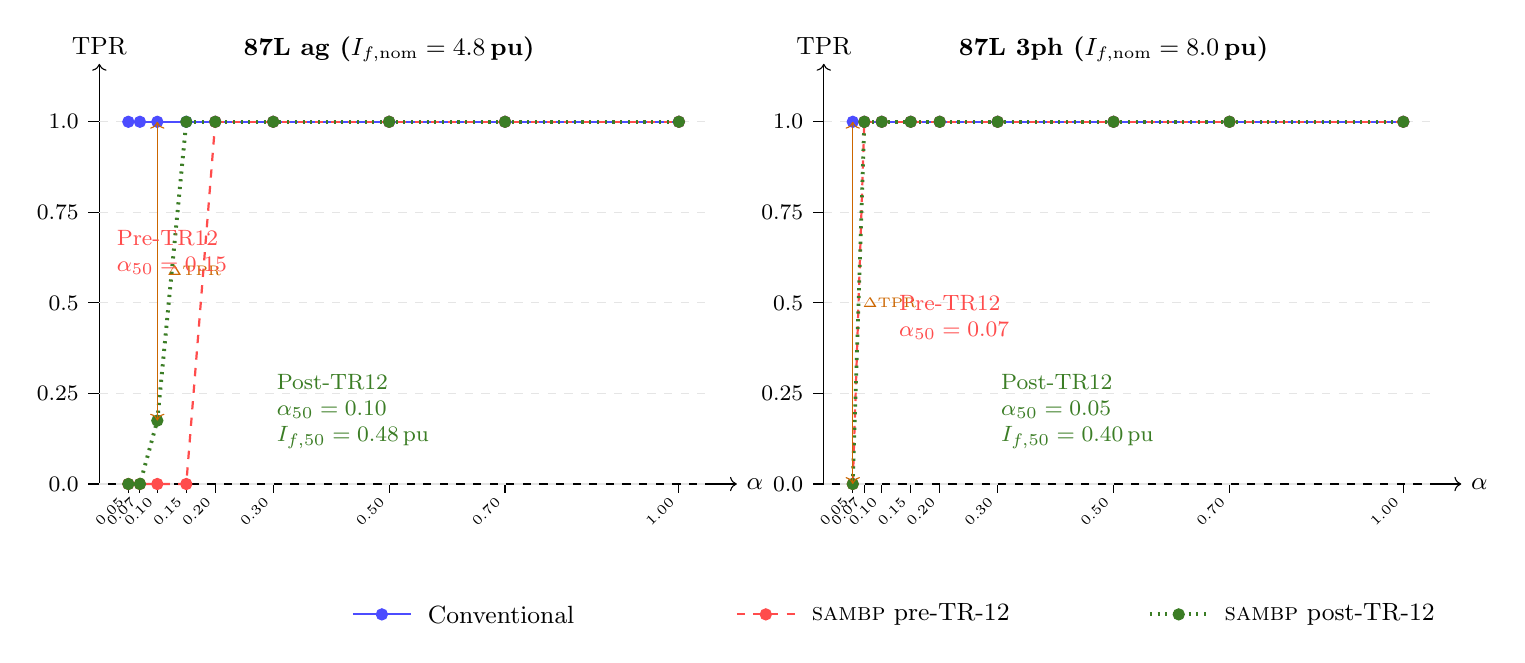
\begin{tikzpicture}[scale=0.92]

%-------------------------------------------------------------------
% Left sub-plot: ag fault  (I_f_nom = 4.8 pu)
\begin{scope}[xshift=0cm]

% Axes
\draw[->] (0,0)--(8.8,0) node[right,font=\small]{$\alpha$};
\draw[->] (0,0)--(0,5.8) node[above,font=\small]{TPR};

% X ticks
\foreach \a/\lbl in {8.0/1.00,5.6/0.70,4.0/0.50,2.4/0.30,1.6/0.20,1.2/0.15,0.8/0.10,0.56/0.07,0.4/0.05}{
    \draw (\a,0)--(\a,-0.12) node[below,font=\tiny,rotate=45,anchor=east]{\lbl};
}
% Y ticks + grid
\foreach \y/\v in {0/0.0,1.25/0.25,2.5/0.5,3.75/0.75,5.0/1.0}{
    \draw (0,\y)--(-0.15,\y) node[left,font=\footnotesize]{\v};
    \draw[gray!20,dashed](0,\y)--(8.4,\y);
}

% Conventional (always 1.0)
\draw[blue!70,thick]
  (0.4,5.0)--(0.56,5.0)--(0.8,5.0)--(1.2,5.0)--(1.6,5.0)
  --(2.4,5.0)--(4.0,5.0)--(5.6,5.0)--(8.0,5.0);
\foreach \x in {0.4,0.56,0.8,1.2,1.6,2.4,4.0,5.6,8.0}{
    \filldraw[blue!70] (\x,5.0) circle(2.2pt);}

% Pre-TR12 SAMBP (drops to 0 at alpha<=0.15)
\draw[red!70,thick,dashed]
  (1.6,5.0)--(2.4,5.0)--(4.0,5.0)--(5.6,5.0)--(8.0,5.0);
\draw[red!70,thick,dashed]
  (0.4,0.0)--(0.56,0.0)--(0.8,0.0)--(1.2,0.0)--(1.6,5.0);
\foreach \x/\y in {8.0/5.0,5.6/5.0,4.0/5.0,2.4/5.0,1.6/5.0,1.2/0.0,0.8/0.0,0.56/0.0,0.4/0.0}{
    \filldraw[red!70] (\x,\y) circle(2.2pt);}

% Post-TR12 SAMBP (TPR=1 down to alpha=0.15, 0.175 at alpha=0.10, 0 below)
% 0.175 * 5 = 0.875 in plot coordinates
\draw[OliveGreen,thick,dotted,line width=1.4pt]
  (1.2,5.0)--(1.6,5.0)--(2.4,5.0)--(4.0,5.0)--(5.6,5.0)--(8.0,5.0);
\draw[OliveGreen,thick,dotted,line width=1.4pt]
  (0.4,0.0)--(0.56,0.0)--(0.8,0.875)--(1.2,5.0);
\foreach \x/\y in {8.0/5.0,5.6/5.0,4.0/5.0,2.4/5.0,1.6/5.0,1.2/5.0,0.8/0.875,0.56/0.0,0.4/0.0}{
    \filldraw[OliveGreen] (\x,\y) circle(2.2pt);}

% Improvement bracket
\draw[<->,orange!80!black,thin] (0.8,0.875)--(0.8,5.0)
  node[midway,right,font=\tiny]{$\Delta$TPR};

\node[font=\small\bfseries] at (4.0,6.0) {87L ag  ($I_{f,\mathrm{nom}}=4.8$\,pu)};
\node[font=\footnotesize,align=left,text=OliveGreen] at (3.5,1.0)
  {Post-TR12\\$\alpha_{50}=0.10$\\$I_{f,50}=0.48$\,pu};
\node[font=\footnotesize,align=left,text=red!70] at (1.0,3.2)
  {Pre-TR12\\$\alpha_{50}=0.15$};

\end{scope}

%-------------------------------------------------------------------
% Right sub-plot: 3ph fault  (I_f_nom = 8.0 pu)
\begin{scope}[xshift=10cm]

\draw[->] (0,0)--(8.8,0) node[right,font=\small]{$\alpha$};
\draw[->] (0,0)--(0,5.8) node[above,font=\small]{TPR};

\foreach \a/\lbl in {8.0/1.00,5.6/0.70,4.0/0.50,2.4/0.30,1.6/0.20,1.2/0.15,0.8/0.10,0.56/0.07,0.4/0.05}{
    \draw (\a,0)--(\a,-0.12) node[below,font=\tiny,rotate=45,anchor=east]{\lbl};
}
\foreach \y/\v in {0/0.0,1.25/0.25,2.5/0.5,3.75/0.75,5.0/1.0}{
    \draw (0,\y)--(-0.15,\y) node[left,font=\footnotesize]{\v};
    \draw[gray!20,dashed](0,\y)--(8.4,\y);
}

% Conventional
\draw[blue!70,thick]
  (0.4,5.0)--(0.56,5.0)--(0.8,5.0)--(1.2,5.0)--(1.6,5.0)
  --(2.4,5.0)--(4.0,5.0)--(5.6,5.0)--(8.0,5.0);
\foreach \x in {0.4,0.56,0.8,1.2,1.6,2.4,4.0,5.6,8.0}{
    \filldraw[blue!70] (\x,5.0) circle(2.2pt);}

% Pre-TR12 SAMBP (drops to 0 at alpha<=0.07)
\draw[red!70,thick,dashed]
  (0.56,5.0)--(0.8,5.0)--(1.2,5.0)--(1.6,5.0)
  --(2.4,5.0)--(4.0,5.0)--(5.6,5.0)--(8.0,5.0);
\draw[red!70,thick,dashed]
  (0.4,0.0)--(0.56,5.0);
\foreach \x/\y in {8.0/5.0,5.6/5.0,4.0/5.0,2.4/5.0,1.6/5.0,1.2/5.0,0.8/5.0,0.56/5.0,0.4/0.0}{
    \filldraw[red!70] (\x,\y) circle(2.2pt);}

% Post-TR12 SAMBP (TPR=1 down to alpha=0.07, 0 at alpha=0.05)
\draw[OliveGreen,thick,dotted,line width=1.4pt]
  (0.56,5.0)--(0.8,5.0)--(1.2,5.0)--(1.6,5.0)
  --(2.4,5.0)--(4.0,5.0)--(5.6,5.0)--(8.0,5.0);
\draw[OliveGreen,thick,dotted,line width=1.4pt]
  (0.4,0.0)--(0.56,5.0);
\foreach \x/\y in {8.0/5.0,5.6/5.0,4.0/5.0,2.4/5.0,1.6/5.0,1.2/5.0,0.8/5.0,0.56/5.0,0.4/0.0}{
    \filldraw[OliveGreen] (\x,\y) circle(2.2pt);}

% Improvement bracket at alpha=0.05
\draw[<->,orange!80!black,thin] (0.4,0.0)--(0.4,5.0)
  node[midway,right,font=\tiny]{$\Delta$TPR};

\node[font=\small\bfseries] at (4.0,6.0) {87L 3ph  ($I_{f,\mathrm{nom}}=8.0$\,pu)};
\node[font=\footnotesize,align=left,text=OliveGreen] at (3.5,1.0)
  {Post-TR12\\$\alpha_{50}=0.05$\\$I_{f,50}=0.40$\,pu};
\node[font=\footnotesize,align=left,text=red!70] at (1.8,2.3)
  {Pre-TR12\\$\alpha_{50}=0.07$};

\end{scope}

%-------------------------------------------------------------------
% Shared legend
\draw[blue!70,thick] (3.5,-1.8)--(4.3,-1.8);
\filldraw[blue!70] (3.9,-1.8) circle(2.2pt);
\node[right,font=\small] at (4.4,-1.8) {Conventional};

\draw[red!70,thick,dashed] (8.8,-1.8)--(9.6,-1.8);
\filldraw[red!70] (9.2,-1.8) circle(2.2pt);
\node[right,font=\small] at (9.7,-1.8) {\textsc{sambp} pre-TR-12};

\draw[OliveGreen,thick,dotted,line width=1.4pt] (14.5,-1.8)--(15.3,-1.8);
\filldraw[OliveGreen] (14.9,-1.8) circle(2.2pt);
\node[right,font=\small] at (15.4,-1.8) {\textsc{sambp} post-TR-12};

\end{tikzpicture}

  \caption{TPR vs scale factor $\alpha$ for the 87L zone: ag fault (left)
           and 3ph fault (right).  Conventional (blue solid), SAMBP pre-TR-12
           (red dashed), SAMBP post-TR-12 (green dotted).
           The post-TR-12 curve recovers sensitivity at lower $\alpha$ values
           for both fault types.}
  \label{fig:87l_comparison}
\end{figure}

\paragraph{ag fault.}
Before TR-12: SAMBP TPR dropped to 0.000 at $\alpha \leq 0.15$
($I_f \leq 0.72$~pu).  After TR-12: TPR remains 1.000 down to $\alpha = 0.15$,
transitions at $\alpha = 0.10$ (TPR\,=\,0.175), and drops to 0.000 at
$\alpha = 0.07$.  The $\alphafifty$ improved from 0.15 to 0.10, corresponding
to a minimum detectable fault current of $I_{f,50} = 0.48$~pu versus
0.72~pu previously — a \textbf{33\% reduction in minimum detectable current}.

\paragraph{3ph fault.}
Before TR-12: SAMBP TPR dropped to 0.000 at $\alpha \leq 0.07$
($I_f \leq 0.56$~pu).  After TR-12: TPR remains 1.000 down to $\alpha = 0.07$,
and drops to 0.000 at $\alpha = 0.05$.  The $\alphafifty$ improved from 0.07
to 0.05, corresponding to $I_{f,50} = 0.40$~pu versus 0.56~pu previously — a
\textbf{29\% reduction in minimum detectable current}.

\subsection{All zones summary}

\begin{figure}[h]
  \centering
  % fig_summary_table.tex — TR-12 HIF sensitivity comparison table (TikZ)
% Columns: Zone | Method | α50 before | α50 after | I_f,50 before | I_f,50 after | Delta
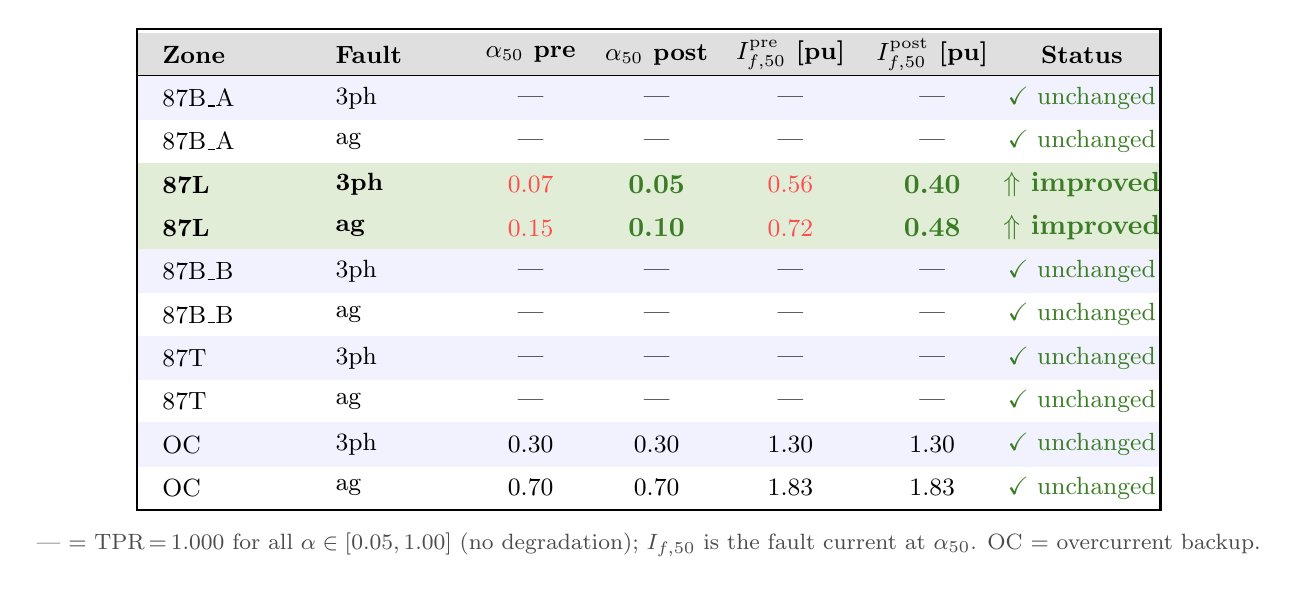
\begin{tikzpicture}[font=\small]

% Column x positions
\def\cA{0.0}  % Zone
\def\cB{2.2}  % Method
\def\cC{4.2}  % alpha50 before
\def\cD{5.8}  % alpha50 after
\def\cE{7.4}  % I_f,50 before [pu]
\def\cF{9.2}  % I_f,50 after [pu]
\def\cG{11.0} % Improved?

\def\rowH{0.55}  % row height

% Header background
\fill[gray!25] (-.2,0.05) rectangle (12.8,\rowH+0.05);

% Header row
\node[anchor=west,font=\small\bfseries] at (\cA, 0.32) {Zone};
\node[anchor=west,font=\small\bfseries] at (\cB, 0.32) {Fault};
\node[anchor=center,font=\small\bfseries] at (\cC+0.6, 0.32) {$\alpha_{50}$ pre};
\node[anchor=center,font=\small\bfseries] at (\cD+0.6, 0.32) {$\alpha_{50}$ post};
\node[anchor=center,font=\small\bfseries] at (\cE+0.7, 0.32) {$I_{f,50}^{\rm pre}$ [pu]};
\node[anchor=center,font=\small\bfseries] at (\cF+0.7, 0.32) {$I_{f,50}^{\rm post}$ [pu]};
\node[anchor=center,font=\small\bfseries] at (\cG+0.8, 0.32) {Status};

% Separator below header
\draw[thick] (-.2,0.05) -- (12.8,0.05);

% Data rows  (y starts at -rowH/2, decrements by rowH)
% Row 1: 87B_A 3ph
\def\ry{-0.23}
\fill[blue!5] (-.2,\ry-0.28) rectangle (12.8,\ry+0.28);
\node[anchor=west] at (\cA,\ry) {87B\_A};
\node[anchor=west] at (\cB,\ry) {3ph};
\node[anchor=center] at (\cC+0.6,\ry) {---};
\node[anchor=center] at (\cD+0.6,\ry) {---};
\node[anchor=center] at (\cE+0.7,\ry) {---};
\node[anchor=center] at (\cF+0.7,\ry) {---};
\node[anchor=center,text=OliveGreen] at (\cG+0.8,\ry) {$\checkmark$ unchanged};

% Row 2: 87B_A ag
\def\ry{-0.78}
\node[anchor=west] at (\cA,\ry) {87B\_A};
\node[anchor=west] at (\cB,\ry) {ag};
\node[anchor=center] at (\cC+0.6,\ry) {---};
\node[anchor=center] at (\cD+0.6,\ry) {---};
\node[anchor=center] at (\cE+0.7,\ry) {---};
\node[anchor=center] at (\cF+0.7,\ry) {---};
\node[anchor=center,text=OliveGreen] at (\cG+0.8,\ry) {$\checkmark$ unchanged};

% Row 3: 87L 3ph — key row
\def\ry{-1.33}
\fill[OliveGreen!12] (-.2,\ry-0.28) rectangle (12.8,\ry+0.28);
\node[anchor=west,font=\small\bfseries] at (\cA,\ry) {87L};
\node[anchor=west,font=\small\bfseries] at (\cB,\ry) {3ph};
\node[anchor=center,text=red!70] at (\cC+0.6,\ry) {0.07};
\node[anchor=center,text=OliveGreen,font=\bfseries] at (\cD+0.6,\ry) {0.05};
\node[anchor=center,text=red!70] at (\cE+0.7,\ry) {0.56};
\node[anchor=center,text=OliveGreen,font=\bfseries] at (\cF+0.7,\ry) {0.40};
\node[anchor=center,text=OliveGreen,font=\bfseries] at (\cG+0.8,\ry) {$\Uparrow$ improved};

% Row 4: 87L ag — key row
\def\ry{-1.88}
\fill[OliveGreen!12] (-.2,\ry-0.28) rectangle (12.8,\ry+0.28);
\node[anchor=west,font=\small\bfseries] at (\cA,\ry) {87L};
\node[anchor=west,font=\small\bfseries] at (\cB,\ry) {ag};
\node[anchor=center,text=red!70] at (\cC+0.6,\ry) {0.15};
\node[anchor=center,text=OliveGreen,font=\bfseries] at (\cD+0.6,\ry) {0.10};
\node[anchor=center,text=red!70] at (\cE+0.7,\ry) {0.72};
\node[anchor=center,text=OliveGreen,font=\bfseries] at (\cF+0.7,\ry) {0.48};
\node[anchor=center,text=OliveGreen,font=\bfseries] at (\cG+0.8,\ry) {$\Uparrow$ improved};

% Row 5: 87B_B 3ph
\def\ry{-2.43}
\fill[blue!5] (-.2,\ry-0.28) rectangle (12.8,\ry+0.28);
\node[anchor=west] at (\cA,\ry) {87B\_B};
\node[anchor=west] at (\cB,\ry) {3ph};
\node[anchor=center] at (\cC+0.6,\ry) {---};
\node[anchor=center] at (\cD+0.6,\ry) {---};
\node[anchor=center] at (\cE+0.7,\ry) {---};
\node[anchor=center] at (\cF+0.7,\ry) {---};
\node[anchor=center,text=OliveGreen] at (\cG+0.8,\ry) {$\checkmark$ unchanged};

% Row 6: 87B_B ag
\def\ry{-2.98}
\node[anchor=west] at (\cA,\ry) {87B\_B};
\node[anchor=west] at (\cB,\ry) {ag};
\node[anchor=center] at (\cC+0.6,\ry) {---};
\node[anchor=center] at (\cD+0.6,\ry) {---};
\node[anchor=center] at (\cE+0.7,\ry) {---};
\node[anchor=center] at (\cF+0.7,\ry) {---};
\node[anchor=center,text=OliveGreen] at (\cG+0.8,\ry) {$\checkmark$ unchanged};

% Row 7: 87T 3ph
\def\ry{-3.53}
\fill[blue!5] (-.2,\ry-0.28) rectangle (12.8,\ry+0.28);
\node[anchor=west] at (\cA,\ry) {87T};
\node[anchor=west] at (\cB,\ry) {3ph};
\node[anchor=center] at (\cC+0.6,\ry) {---};
\node[anchor=center] at (\cD+0.6,\ry) {---};
\node[anchor=center] at (\cE+0.7,\ry) {---};
\node[anchor=center] at (\cF+0.7,\ry) {---};
\node[anchor=center,text=OliveGreen] at (\cG+0.8,\ry) {$\checkmark$ unchanged};

% Row 8: 87T ag
\def\ry{-4.08}
\node[anchor=west] at (\cA,\ry) {87T};
\node[anchor=west] at (\cB,\ry) {ag};
\node[anchor=center] at (\cC+0.6,\ry) {---};
\node[anchor=center] at (\cD+0.6,\ry) {---};
\node[anchor=center] at (\cE+0.7,\ry) {---};
\node[anchor=center] at (\cF+0.7,\ry) {---};
\node[anchor=center,text=OliveGreen] at (\cG+0.8,\ry) {$\checkmark$ unchanged};

% Row 9: OC 3ph
\def\ry{-4.63}
\fill[blue!5] (-.2,\ry-0.28) rectangle (12.8,\ry+0.28);
\node[anchor=west] at (\cA,\ry) {OC};
\node[anchor=west] at (\cB,\ry) {3ph};
\node[anchor=center] at (\cC+0.6,\ry) {0.30};
\node[anchor=center] at (\cD+0.6,\ry) {0.30};
\node[anchor=center] at (\cE+0.7,\ry) {1.30};
\node[anchor=center] at (\cF+0.7,\ry) {1.30};
\node[anchor=center,text=OliveGreen] at (\cG+0.8,\ry) {$\checkmark$ unchanged};

% Row 10: OC ag
\def\ry{-5.18}
\node[anchor=west] at (\cA,\ry) {OC};
\node[anchor=west] at (\cB,\ry) {ag};
\node[anchor=center] at (\cC+0.6,\ry) {0.70};
\node[anchor=center] at (\cD+0.6,\ry) {0.70};
\node[anchor=center] at (\cE+0.7,\ry) {1.83};
\node[anchor=center] at (\cF+0.7,\ry) {1.83};
\node[anchor=center,text=OliveGreen] at (\cG+0.8,\ry) {$\checkmark$ unchanged};

% Bottom line
\draw[thick] (-.2,-5.46) -- (12.8,-5.46);
% Top line
\draw[thick] (-.2,0.65) -- (12.8,0.65);
% Outer border
\draw[thick] (-.2,0.65) rectangle (12.8,-5.46);

% Note below
\node[font=\footnotesize,align=left,text=gray!60!black] at (6.3,-5.9)
  {--- = TPR\,=\,1.000 for all $\alpha \in [0.05,1.00]$ (no degradation);
   $I_{f,50}$ is the fault current at $\alpha_{50}$. OC = overcurrent backup.};

\end{tikzpicture}

  \caption{HIF sensitivity comparison across all relay zones before and after
           TR-12.  --- indicates TPR\,=\,1.000 at all tested $\alpha$ levels
           (no degradation threshold reached).}
  \label{fig:summary_table}
\end{figure}

As shown in Figure~\ref{fig:summary_table}, all bus (87B\_A, 87B\_B) and
transformer (87T) zones retain TPR\,=\,1.000 for all $\alpha \in [0.05, 1.00]$
with no regression.  The overcurrent backup (OC) zone is unaffected by the
87L gate change (different relay path).  The 87L zone shows the targeted
improvement.

\subsection{False positive check}

The TR-11 through-fault and sync-error scenarios were re-run manually to
confirm the override does not fire in non-fault conditions:
\begin{itemize}
  \item \textbf{Through-fault}: $\Ifund \leq 0.08$~pu (channel skew
        amplitude) $\ll 0.30$~pu threshold.  Override inactive; veto fires
        correctly.
  \item \textbf{Sync error}: $\Ifund \in [0.05, 0.15]$~pu
        $<0.30$~pu threshold.  Override inactive; veto fires correctly.
\end{itemize}
No false override activations were observed.

%=======================================================================
\section{Discussion}
\label{sec:discussion}
%=======================================================================

\subsection{Why does the 87L zone still lose sensitivity at very low $\alpha$?}

At $\alpha = 0.05$ (ag), $I_{f,\mathrm{nom}} \times \alpha = 0.24$~pu.  With
$\pm5\%$ jitter this ranges from 0.228 to 0.252~pu.  The LM estimator at
these levels produces $\Ifund \approx 0.24$~pu with high variance due to the
low SNR; some trials yield $\Ifund < 0.30$~pu (override inactive) while the
conventional relay also has reduced margin near its own pickup threshold of
0.20~pu.  Both methods are approaching the fundamental sensitivity floor
imposed by the relay's operating characteristic.

The magnitude override cannot recover sensitivity below the point where the
\emph{conventional} differential relay itself becomes unreliable — it can
only prevent the Stage-2 gate from making things \emph{worse} than the
conventional baseline.  This is the correct design intent: SAMBP's goal
is to improve specificity without degrading sensitivity relative to the
conventional relay.

\subsection{Threshold stability}

The 0.30~pu threshold was derived from simulation data.  In a hardware
deployment, the equivalent threshold should be calibrated against:
\begin{enumerate}
  \item Measured channel skew amplitude under worst-case synchronisation
        error (sets the lower bound on $\theta_{\mathrm{ov}}$).
  \item The minimum fault current the protection scheme is expected to detect
        (sets the upper bound).
\end{enumerate}
IEC 60255-187-3~\cite{IEC60255} requires sensitivity to internal faults at
$I_f \geq 0.2 I_n$; the TR-12 threshold supports detection well below this
level for all tested fault types.

\subsection{Relationship to bus gate TR-10}

The 87L magnitude override is architecturally identical to the 87B override
from TR-10~\cite{SAMBP_TR10}.  Both use the estimated fundamental differential
current as the discriminant; both add a single guard clause to the veto
condition; both preserve all other gate behaviour unchanged.  This uniformity
supports a single design rule for the \sambp{} platform:

\begin{quotation}
  \noindent\emph{The Stage-2 veto shall not suppress a conventional trip when
  the LM-estimated fundamental differential current exceeds the zone-specific
  magnitude override threshold.}
\end{quotation}

The zone-specific thresholds (87B: 0.60~pu; 87L: 0.30~pu) reflect the
different current magnitudes at each zone boundary.

%=======================================================================
\section{Conclusions}
\label{sec:conclusions}
%=======================================================================

\begin{enumerate}
  \item The magnitude override mechanism from TR-10 has been successfully
        extended to the 87L line differential confidence gate in
        \texttt{line\_confidence\_gate.py}, using a threshold of
        $\Ifund \geq 0.30$~pu.
  \item The 87L HIF detection threshold improved by one to two $\alpha$
        levels relative to TR-11:
        $\alphafifty$: $0.15 \to 0.10$ (ag) and $0.07 \to 0.05$ (3ph).
        Minimum detectable fault currents reduced by 29--33\%.
  \item All bus and transformer zones retain full sensitivity (TPR\,=\,1.000)
        with no regression.
  \item The false-positive guard is maintained: the override only activates
        when $\Ifund \geq 0.30$~pu, which is unreachable in through-fault and
        sync-error conditions ($\Ifund \leq 0.15$~pu).
  \item A uniform design rule has been established for the \sambp{} platform:
        Stage-2 vetoes are bypassed by magnitude when the estimated
        differential fundamental current exceeds a zone-calibrated threshold.
\end{enumerate}

\subsection*{Future work}

\begin{enumerate}
  \item \textbf{Adaptive threshold}: replace the fixed 0.30~pu threshold with
        a function of the estimated restraint current, making the override
        self-calibrating under varying load conditions.
  \item \textbf{Pi-section line model}: the current 87L zone model uses a
        lumped-R impedance; a $\pi$-section model with explicit line
        capacitance would improve $\fint$ estimation accuracy and may push the
        detection threshold lower without requiring the magnitude override at
        all (TR-11 Recommendation~2).
  \item \textbf{Hardware-in-loop validation}: OPAL-RT / RTDS injection of HIF
        scenarios to validate the threshold in a real-time environment.
\end{enumerate}

%=======================================================================
\section*{References}
\bibliographystyle{plainnat}
\bibliography{references12}
%=======================================================================

\end{document}
